% SC4064 --- Chapter 2: CUDA Threads, Blocks, Grids and Kernels (0->100 ground-up)
\chapter{CUDA Threads, Blocks, Grids and Kernels}
\label{ch:cuda}
\sloppy

\begin{quote}
\emph{``A kernel is a single program executed by thousands of threads, each knowing who it is.''} The CUDA hierarchy---thread, block, grid---is how you name those threads and map them to data. Master the mapping and every kernel becomes bookkeeping; miss it and you read the wrong element or launch the wrong count.
\end{quote}

\noindent\fbox{\parbox{\dimexpr\linewidth-2\fboxsep-2\fboxrule}{%
\textbf{From zero: no CUDA background assumed.} We build from a sequential loop to a parallel kernel step by step: what \texttt{\_\_global\_\_} means, why we need blocks and grids, how \texttt{threadIdx} and \texttt{blockIdx} give a global identity, and how warps (Ch.~1) map under the hood. Every index formula is derived, not memorised.}}
\vspace{0.4em}

\section*{Learning Outcomes}
After this chapter you will be able to:
\begin{enumerate}[label=(L\arabic*)]
    \item write and launch a CUDA kernel with correct \texttt{\_\_\_global\_\_\_} and \texttt{<<<grid,block>>>} syntax;
    \item compute 1-D and 2-D global thread indices from \texttt{threadIdx}, \texttt{blockIdx}, \texttt{blockDim}, \texttt{gridDim};
    \item explain the block--SM mapping, why block size matters, and the limits (1024 threads/block, 32 warps/SM);
    \item use \texttt{\_\_syncthreads()} correctly and state what it does and does not synchronise;
    \item size grids with the ceil division $(n+B-1)/B$ and guard out-of-bounds accesses.
\end{enumerate}

% ============================================================
\section{From Loop to Kernel: The Launch Hierarchy}
\label{sec:launch-hierarchy}
\paragraph{Intuition.} A sequential loop says ``for $i=0$ to $n-1$ do $c[i]=a[i]+b[i]$'' and one thread walks $i$ step by step. A CUDA kernel flips this: it says ``I am thread $i$; I do $c[i]=a[i]+b[i]$ for my $i$'' and a million threads run that sentence simultaneously, each with a different $i$. The hierarchy tells each thread what its $i$ is.

CUDA exposes three levels. A \emph{thread} executes one instance of the kernel. Threads are grouped into a \emph{block} (up to 1024 threads, 1-D/2-D/3-D shape) that runs on one SM and can cooperate via shared memory and \texttt{\_\_syncthreads()}. Blocks are grouped into a \emph{grid} (1-D/2-D/3-D) that spans the whole device; blocks are independent and may run in any order on any SM. The programmer chooses block shape; the hardware maps blocks to SMs.

\begin{definition}[Kernel, block, grid]
A \emph{kernel} is a function marked \texttt{\_\_global\_\_} executed $N$ times in parallel by $N$ threads. A \emph{block} is a cooperating group of threads (max 1024) on one SM. A \emph{grid} is the collection of blocks launched for one kernel. Built-ins \texttt{threadIdx}, \texttt{blockIdx}, \texttt{blockDim}, \texttt{gridDim} give position and size at each level.
\end{definition}

\begin{figure}[h]\centering
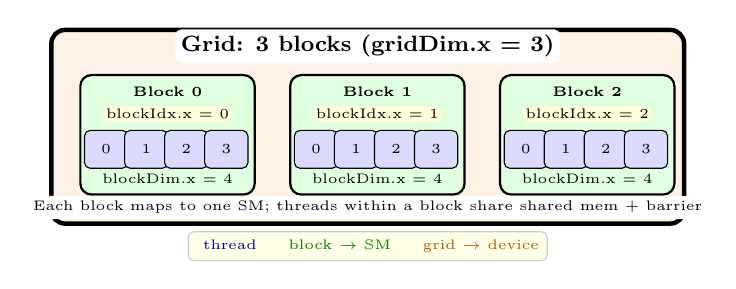
\begin{tikzpicture}[scale=0.82, every node/.style={font=\scriptsize},
  thr/.style={draw, rounded corners=2pt, minimum width=0.55cm, minimum height=0.48cm, fill=blue!14},
  blk/.style={draw, thick, rounded corners=4pt, fill=green!12},
  grd/.style={draw, ultra thick, rounded corners=5pt, fill=orange!10}]
% Grid
\draw[grd] (-0.3,-0.4) rectangle (9.5,2.6);
\node[font=\footnotesize\bfseries, fill=white, rounded corners=2pt, inner sep=2pt] at (4.6,2.35) {Grid: 3 blocks (gridDim.x = 3)};
% Blocks
\foreach \bx in {0,3.25,6.5} {
  \draw[blk] (\bx+0.15,0.05) rectangle (\bx+2.85,1.90);
  \node[font=\tiny\bfseries] at (\bx+1.5,1.65) {Block \pgfmathparse{int(\bx/3.25)}\pgfmathresult};
  \node[font=\tiny, fill=yellow!15, rounded corners=2pt, inner sep=1pt] at (\bx+1.5,1.30) {blockIdx.x = \pgfmathparse{int(\bx/3.25)}\pgfmathresult};
  % threads as small boxes
  \foreach \tx in {0,0.62,1.24,1.86} {
    \node[thr] at (\bx+0.55+\tx,0.75) {\tiny \pgfmathparse{int(\tx/0.62)}\pgfmathresult};
  }
  \node[font=\tiny] at (\bx+1.5,0.30) {blockDim.x = 4};
}
\node[font=\tiny, align=center, fill=white, rounded corners=2pt, inner sep=2pt] at (4.6,-0.15) {Each block maps to one SM; threads within a block share shared mem + barrier};
\node[font=\tiny, align=left, fill=yellow!10, draw=gray!40, rounded corners=2pt, inner sep=3pt] at (4.6,-0.75) {\textcolor{blue!60!black}{$\blacksquare$ thread} \quad \textcolor{green!50!black}{$\blacksquare$ block $\to$ SM} \quad \textcolor{orange!70!black}{$\blacksquare$ grid $\to$ device}};
\end{tikzpicture}
\caption{Thread hierarchy: 12 threads organised as $\langle$grid 3 blocks$\rangle \times \langle$block 4 threads$\rangle$. Warps cut across threads (here 1 warp per block for illustration; real warps are 32 threads).}
\label{fig:thread-hierarchy}
\end{figure}

Launching uses triple chevrons: \texttt{kernel<<<gridDim, blockDim>>>(args)}. Both \texttt{gridDim} and \texttt{blockDim} may be \texttt{int}, \texttt{dim3(x)}, or \texttt{dim3(x,y,z)}. Inside, \texttt{threadIdx.x} ranges $0\ldots$\texttt{blockDim.x}$-1$, \texttt{blockIdx.x} ranges $0\ldots$\texttt{gridDim.x}$-1$. The next section derives the global index.

% ============================================================
\section{Indexing: Who Am I?}
\label{sec:indexing}
\paragraph{Intuition.} Mailboxes are numbered globally but you only know your street and house number. Global thread id is the mailbox: \texttt{blockIdx}$\times$\texttt{blockDim} $+$ \texttt{threadIdx}. For 2-D data (images, matrices) the same idea extends to rows and columns.

For 1-D, with \texttt{blockDim.x}=256:
\begin{equation}
\texttt{tid} = \texttt{blockIdx.x}\times\texttt{blockDim.x} + \texttt{threadIdx.x}.
\end{equation}
For 2-D, with blocks of $B_x\times B_y$ and grid $G_x\times G_y$:
\begin{align}
x &= \texttt{blockIdx.x}\times\texttt{blockDim.x} + \texttt{threadIdx.x},\\
y &= \texttt{blockIdx.y}\times\texttt{blockDim.y} + \texttt{threadIdx.y},\\
\texttt{globalRowMajor} &= y\times\texttt{width} + x.
\end{align}
If total threads exceed $n$, guard with \texttt{if(tid < n) return;}---otherwise out-of-bounds reads corrupt memory silently.

\begin{figure}[h]\centering
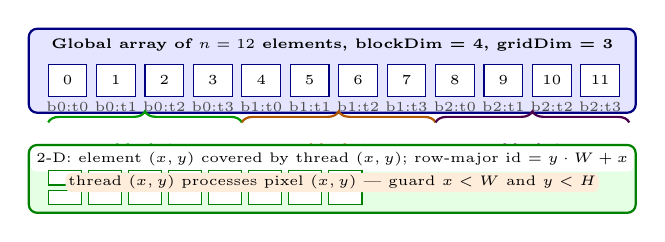
\begin{tikzpicture}[scale=0.82, every node/.style={font=\scriptsize}]
% 1D indexing illustration
\draw[fill=blue!10, draw=blue!50!black, thick, rounded corners=3pt] (0,1.6) rectangle (9.4,2.9);
\node[font=\tiny\bfseries] at (4.7,2.65) {Global array of $n=12$ elements, blockDim = 4, gridDim = 3};
\foreach \i in {0,...,11} {
  \draw[fill=white, draw=blue!50!black] (0.30+\i*0.75,1.85) rectangle (0.90+\i*0.75,2.35);
  \node[font=\tiny] at (0.60+\i*0.75,2.10) {\i};
  \pgfmathtruncatemacro{\blk}{int(\i/4)}
  \pgfmathtruncatemacro{\th}{int(mod(\i,4))}
  \node[font=\tiny, text=gray!60!black] at (0.60+\i*0.75,1.70) {b\blk:t\th};
}
% block grouping brackets
\draw[decorate, decoration={brace, amplitude=4pt}, thick, green!60!black] (0.30,1.45) -- (3.30,1.45) node[midway, below=4pt, font=\tiny] {block 0};
\draw[decorate, decoration={brace, amplitude=4pt}, thick, orange!70!black] (3.30+0.00,1.45) -- (6.30,1.45) node[midway, below=4pt, font=\tiny] {block 1};
\draw[decorate, decoration={brace, amplitude=4pt}, thick, violet!60!black] (6.30+0.00,1.45) -- (9.30,1.45) node[midway, below=4pt, font=\tiny] {block 2};
% 2D grid inset
\draw[fill=green!10, draw=green!50!black, thick, rounded corners=3pt] (0,0.05) rectangle (9.4,1.10);
\node[font=\tiny, fill=white, rounded corners=2pt, inner sep=2pt] at (4.7,0.88) {2-D: element $(x,y)$ covered by thread $(x,y)$; row-major id $= y\cdot W + x$};
\foreach \y in {0,1} {
  \foreach \x in {0,...,7} {
    \draw[fill=white, draw=green!50!black] (0.30+\x*0.62,0.18+\y*0.30) rectangle (0.82+\x*0.62,0.40+\y*0.30);
  }
}
\node[font=\tiny, fill=orange!14, rounded corners=2pt, inner sep=1pt] at (4.7,0.52) {thread $(x,y)$ processes pixel $(x,y)$ --- guard $x<W$ and $y<H$};
\end{tikzpicture}
\caption{Indexing: 1-D global id as block$\times$blockDim + thread; 2-D extends to $(x,y)$ with row-major linearisation. The brace grouping shows how 12 elements map to 3 blocks of 4.}
\label{fig:indexing}
\end{figure}

\begin{example}[Ceiling division]
To cover $n=1000$ elements with $B=256$ threads/block, need $G=\lceil n/B\rceil = (1000+255)/256 = 4$ blocks (1024 threads). Threads 1000--1023 exist but do no work due to the \texttt{if(tid < n)} guard. For 2-D image $W=1920, H=1080$ with $16\times16$ blocks, $G_x=\lceil1920/16\rceil=120$, $G_y=\lceil1080/16\rceil=68$.
\end{example}

% ============================================================
\section{Warps, Scheduling and Synchronisation}
\label{sec:warps-sync}
Hardware groups threads into warps of 32 consecutive \texttt{threadIdx.x} values (then wraps to next row for 2-D). Warps are the scheduling unit on the SM (Ch.~1). A warp scheduler picks a ready warp each cycle; if one warp stalls on memory, another runs---latency hiding. This is why occupancy (many resident warps, Ch.~4) matters even when indexing looks correct.

\begin{figure}[h]\centering
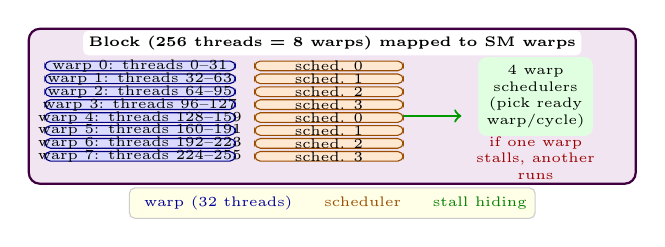
\begin{tikzpicture}[scale=0.82, every node/.style={font=\scriptsize}]
\draw[fill=violet!10, draw=violet!50!black, thick, rounded corners=4pt] (0,0) rectangle (9.4,2.4);
\node[font=\tiny\bfseries, fill=white, rounded corners=2pt, inner sep=2pt] at (4.7,2.18) {Block (256 threads = 8 warps) mapped to SM warps};
\foreach \w in {0,...,7} {
  \draw[fill=blue!14, draw=blue!50!black, rounded corners=2pt] (0.25,1.75-\w*0.20) rectangle (3.20,1.90-\w*0.20);
  \node[font=\tiny, align=left] at (1.72,1.825-\w*0.20) {warp \w: threads \pgfmathparse{int(\w*32)}\pgfmathresult--\pgfmathparse{int(\w*32+31)}\pgfmathresult};
  \draw[fill=orange!18, draw=orange!60!black, rounded corners=2pt] (3.50,1.75-\w*0.20) rectangle (5.80,1.90-\w*0.20);
  \node[font=\tiny] at (4.65,1.825-\w*0.20) {sched. \pgfmathparse{int(mod(\w,4))}\pgfmathresult};
}
\node[font=\tiny, align=center, fill=green!12, rounded corners=3pt, inner sep=3pt] at (7.85,1.35) {4 warp\\schedulers\\(pick ready\\warp/cycle)};
\draw[->, thick, green!60!black] (5.80,1.05) -- (6.70,1.05);
\node[font=\tiny, text=red!60!black, align=center] at (7.85,0.40) {if one warp\\stalls, another\\runs};
\node[font=\tiny, align=left, fill=yellow!10, draw=gray!40, rounded corners=2pt, inner sep=3pt] at (4.7,-0.30) {\textcolor{blue!60!black}{$\blacksquare$ warp (32 threads)} \quad \textcolor{orange!60!black}{$\blacksquare$ scheduler} \quad \textcolor{green!50!black}{$\blacksquare$ stall hiding}};
\end{tikzpicture}
\caption{Warps within a block: 256 threads become 8 warps; 4 schedulers pick among ready warps each cycle. Thread-to-warp mapping is fixed: consecutive threadIdx group into warps.}
\label{fig:warp-sched}
\end{figure}

\paragraph{Synchronisation.} \texttt{\_\_syncthreads()} is a block-wide barrier: no thread passes it until all threads in the block have arrived. It is essential when threads share data via shared memory (Ch.~3): write, barrier, then read. It does \emph{not} synchronise across blocks---blocks are independent; for grid-wide sync use \texttt{cudaDeviceSynchronize()} on the host or cooperative groups. Placing \texttt{\_\_syncthreads()} inside divergent branches causes deadlock (some threads never arrive); keep barriers uniform.

\begin{remark}[Common indexing bugs]
Off-by-one in ceil division ($n/B$ instead of $(n+B-1)/B$) misses the tail. Forgetting the guard writes past the array. Swapping \texttt{blockIdx} and \texttt{threadIdx} scrambles order. Mixing \texttt{blockDim.x} with \texttt{gridDim.x} gives the wrong stride. When in doubt, print \texttt{tid} for a tiny $n$ and check the mapping on paper before scaling.
\end{remark}

\begin{example}[Launch configurator pattern]
Wrap ceil division in a helper: \texttt{dim3 ceilDiv(dim3 n, dim3 B)\{return \{(n.x+B.x-1)/B.x,(n.y+B.y-1)/B.y\};\}}. Then \texttt{grid = ceilDiv(\{W,H\},\{16,16\})}. This avoids copy-pasted arithmetic and makes 1-D/2-D/3-D consistent. Always assert \texttt{grid.x*block.x >= n} in debug builds---a cheap check that catches the most common launch bug.
\end{example}

\smallskip

\begin{lstlisting}[language=C++, caption={Complete 1-D vector addition: device kernel, host launch with ceil division and guard.}, label={lst:vecadd-cuda}]
__global__ void vecAdd(const float *a, const float *b, float *c, int n){
    int tid = blockIdx.x * blockDim.x + threadIdx.x; // global 1-D id
    if(tid < n) c[tid] = a[tid] + b[tid];             // guard tail
}
int main(){
    int n = 1<<20; // 1M elements
    float *d_a,*d_b,*d_c;
    cudaMalloc(&d_a, n*sizeof(float));
    cudaMalloc(&d_b, n*sizeof(float));
    cudaMalloc(&d_c, n*sizeof(float));
    int B = 256;                     // threads per block (tunable, Ch.4)
    int G = (n + B - 1)/B;           // ceil(n/B) blocks
    vecAdd<<<G, B>>>(d_a, d_b, d_c, n);
    cudaDeviceSynchronize();         // wait for grid to finish
    // cudaMemcpy back, check, free ...
}
\end{lstlisting}

\begin{lstlisting}[language=C++, caption={2-D kernel: RGB image grayscale. Each thread handles one pixel $(x,y)$.}, label={lst:kernel2d}]
__global__ void rgb2gray(unsigned char *img, unsigned char *gray, int W, int H){
    int x = blockIdx.x * blockDim.x + threadIdx.x; // column
    int y = blockIdx.y * blockDim.y + threadIdx.y; // row
    if(x >= W || y >= H) return;                   // 2-D guard
    int idx = y * W + x;                           // row-major
    unsigned char r = img[3*idx], g = img[3*idx+1], b = img[3*idx+2];
    gray[idx] = (unsigned char)(0.299f*r + 0.587f*g + 0.114f*b);
}
int main2(){
    int W=1920, H=1080;
    dim3 block(16,16); // 256 threads/block
    dim3 grid((W+15)/16, (H+15)/16); // 120 x 68
    // rgb2gray<<<grid, block>>>(d_img, d_gray, W, H);
    return 0;
}
\end{lstlisting}

% ============================================================
\section{Exercises}
\label{sec:ch02-exercises}
\begin{enumerate}[label=E2.\arabic*, leftmargin=*, itemsep=0.6em]
    \item \textbf{Index arithmetic.} With \texttt{blockDim.x}=128 and \texttt{blockIdx.x}=5, \texttt{threadIdx.x}=17, what is \texttt{tid}? If $n=700$ and $B=128$, compute $G$ and list which \texttt{tid} values are guarded out. What happens if you forget the guard?
    \item \textbf{2-D launch.} An image is $640\times480$, block is $16\times16$. Compute $G_x, G_y$ and total threads launched. How many threads are idle? Write the 2-D global $(x,y)$ and linear index formulas.
    \item \textbf{Block size limits.} Why cannot a block have 2048 threads even if the SM holds 2048? Explain the 1024 limit and give two reasons a smaller block (e.g., 256) is often faster despite launching more blocks.
    \item \textbf{Barrier correctness.} A kernel does: \texttt{shared[tid]=data[tid]; if(tid\%2==0) \_\_syncthreads(); y=shared[tid+1];}. Why can this deadlock or give wrong answers? Fix it and explain where \texttt{\_\_syncthreads()} must be placed.
    \item \textbf{Warp mapping.} A block is $32\times8$ (256 threads, \texttt{threadIdx} 2-D). Which threads belong to warp 0, warp 1? Does 2-D thread layout affect warp grouping? Explain the linearisation order assumed by hardware.
\end{enumerate}

% ============================================================
\section*{Chapter Notes}
CUDA C++ Programming Guide (NVIDIA, v12.x) \S2--3 defines kernels, hierarchy and built-ins precisely; the \texttt{dim3} type and occupancy calculator are documented there. Kirk \& Hwu Ch.~3--4 work many indexing examples. For grid-wide synchronisation see Cooperative Groups (\texttt{cooperative\_groups::grid\_group}). Hwu et~al., \emph{Heterogeneous System Architecture} (Morgan Kaufmann, 2015) contrasts CUDA with OpenCL/HIP hierarchies (work-group/work-item map to block/thread).
% End of Chapter 2
